\documentclass[usenatbib]{mn2e} 
\usepackage{amsmath} 
\usepackage{amssymb} 
\usepackage{graphics}
\usepackage{graphicx}
\usepackage{epsfig}  
\def\be{\begin{equation}}
\def\ee{\end{equation}}
\def\ba{\begin{eqnarray}}
\def\ea{\end{eqnarray}}



\newcommand{\apj}{ApJ}  
\newcommand{\apjs}{ApJS}  
\newcommand{\apjl}{ApJL}  
\newcommand{\aj}{AJ}  
\newcommand{\mnras}{MNRAS}  
\newcommand{\mnrassub}{MNRAS accepted}  
\newcommand{\aap}{A\&A}  
\newcommand{\aaps}{A\&AS}  
\newcommand{\araa}{ARA\&A}  
\newcommand{\nat}{Nature}  
\newcommand{\physrep}{PhR}
\newcommand{\pasp}{PASP}    
\newcommand{\pasj}{PASJ}    

\newcommand{\kms}{\,km~s$^{-1}$}
\def\squig{\sim\!\!}
\newcommand{\LCDM}{$\Lambda$CDM~}
\newcommand{\beq}{\begin{eqnarray}}  
\newcommand{\eeq}{\end{eqnarray}}  
\newcommand{\zz}{$z\sim 3$} 
\newcommand{\avg}[1]{\langle{#1}\rangle}  
\newcommand{\ly}{{\ifmmode{{\rm Ly}\alpha}\else{Ly$\alpha$}\fi}}
\newcommand{\hMpc}{{\ifmmode{h^{-1}{\rm Mpc}}\else{$h^{-1}$Mpc }\fi}}  
\newcommand{\hGpc}{{\ifmmode{h^{-1}{\rm Gpc}}\else{$h^{-1}$Gpc }\fi}}  
\newcommand{\hmpc}{{\ifmmode{h^{-1}{\rm Mpc}}\else{$h^{-1}$Mpc }\fi}}  
\newcommand{\hkpc}{{\ifmmode{h^{-1}{\rm kpc}}\else{$h^{-1}$kpc }\fi}}  
\newcommand{\hMsun}{{\ifmmode{h^{-1}{\rm {M_{\odot}}}}\else{$h^{-1}{\rm{M_{\odot}}}$}\fi}}  
\newcommand{\hmsun}{{\ifmmode{h^{-1}{\rm {M_{\odot}}}}\else{$h^{-1}{\rm{M_{\odot}}}$}\fi}}  
\newcommand{\Msun}{{\ifmmode{{\rm {M_{\odot}}}}\else{${\rm{M_{\odot}}}$}\fi}}  
\newcommand{\msun}{{\ifmmode{{\rm {M_{\odot}}}}\else{${\rm{M_{\odot}}}$}\fi}}  
\newcommand{\lya}{{Lyman$\alpha$~}}
\newcommand{\clara}{{\texttt{CLARA}}~}
\newcommand{\rand}{{\ifmmode{{\mathcal{R}}}\else{${\mathcal{R}}$ }\fi}}  
\newcommand{\Lsun}{\mbox{\,$L_{\odot}$}}
\newcommand{\like}{\mathscr{L}}
\newcommand{\bftheta}{\mathbf{\Theta}}
\newcommand{\degree}{\ensuremath{^\circ}}
\def\spose#1{\hbox to 0pt{#1\hss}}
\def\simlt{\mathrel{\spose{\lower 3pt\hbox{$\mathchar"218$}}
     \raise 2.0pt\hbox{$\mathchar"13C$}}}
\def\simgt{\mathrel{\spose{\lower 3pt\hbox{$\mathchar"218$}}
     \raise 2.0pt\hbox{$\mathchar"13E$}}}
\font\smcap=cmcsc10

\begin{document}

\title[Dark Matter Halo Mass for LAEs  at $z=3.1$]{Constraints on the
  dark matter halo mass of Lyman-alpha emitting galaxies at $z$=3.1
  from cosmic variance} 
\author[J.E. Forero-Romero and J. Mejia]{
\parbox[t]{\textwidth}{\raggedright Jaime E. Forero-Romero$^{1}$ and Julian Mejia$^{2}$}
\vspace*{6pt}\\
$^{1}$\\
$^{2}$
}

\maketitle

\begin{abstract}
In this Letter we implement a new method to find the characteristic
mass of dark matter halos hosting Lyman-Alpha Emitting (LAE)
galaxies. The method is based on matching the statistics for the
cosmic variance with the observations recently obtained by
\cite{Yamada2012}. We build a model for LAEs on top of a large N-body
cosmological simulation (Bolshoi). The basic principle is that a dark
matter halo can host one LAE with a probability $f_{\rm occ}$ if its
mass is found withing a certain range mass range delimited by two
threshold values, $M_{\rm min}$ and $M_{\rm max}$. We generate
hundreds of mock catalogs in a thourough exploration of the parameter
space of this model. These catalogs are constructed in such a way as
to reproduce the spatial correlation between the different observed
fields. We find that the models that best match the observed cosmic
variance statistics are those with halo masses in the range $M_{\rm
  min}=$ and $M_{\rm max}=$ with and occupation fraction that scales
as $f_{\rm occ}=$ with the minimum mass. We find that the angular
correlation function is in agreement with the observational
constraints mostly due to the cosmic variance in the small angular
fields where this statistics has been computed so far. We also present
predictions for future measurements of the correlation function on
larger continous fields. We make available the mock data for the best
models in a public repository.  
\end{abstract}

\begin{keywords}
{galaxies: kinematics and dynamics, Local Group, methods:numerical}
\end{keywords}


\section{Introduction}

Lyman-$\alpha$ emitting galaxies (LAEs) have become in the last decade a 
central topic in studies of structure formation in the Universe. The
reason is the diverse range of fields where they are helpful, LAEs can
be used as probes of reionization, tracers of large scale structure,
signposts for low metallicity stellar populations and markers of the
the galaxy formation process through cosmic history.  


At the same time, theoretical and observational developments have
contributed to the emergence of a paradigm to describe structure
formation in a cosmological context. In this context it is considered
that dominant matter content of the Universe is to be found in dark
matter, whereby each galaxy is hosted by larger dark matter structure
known as a halo. 

Most models of galaxy formation find that the mass of the halo largely
determines key properties of the galaxy such as its stellar mass and
star formation rate. Processes that regulate the star formation cycle
are also though to be strongly dependent on its mass. Furthermore, the
spatial clustering of galaxies on large scales is entirely dictated by
the halo distribution.  For the reasons mentioned above, finding the
typical dark matter halo mass hosting LAEs represents a significant
step forward to understand the nature of this population in the
context of LCDM.  

Some theoretical approaches to this problem have been based on a
forward modelling. Starting from the DM halo population, the
corresponding intrinsic star formation properties are infered and
statistics such as the luminosity function, the correlation function
and the equivalent width distributions. Such modelling has been
implemented from analytic considerations, semi-analytic models and
full N-body hidrodynamical simulations. 

Added to the uncertainties in the astrophysical processeses describing
star formation in galactic populations, a highly debated steps in this
approach is the calculation of the fraction of Lyman-$\alpha$ photons
that escape the galaxy to the observer. Given the resonance nature of
the line, the radiative transfer of Lyman-$\alpha$ is sensitive to the
density, temperature, topology and kinematics of the neutral Hydrogen
in the interstellar medium (ISM).  

This complexity makes the use of monte-carlo simulations for the
radiative transfer a required tool to obtain physically sound results,
although the degeneracy in the physical parameters involved in the
problem makes it difficult to achieve a robust consensus on what is
the theoretical expected value for the Lyman-$alpha$ escape fraction
in high redshift. 


Throughout this Letter we assume a $\Lambda$CDM cosmology with the
following values for the cosmological parameters, $\Omega_{m}=0.27$,
$\Omega_{\Lambda}=0.73$ and $h=0.70$, corresponding to the matter
density, vacuum density and the Hubble constant in units of 100 km
s$^{-1}$ Mpc$^{-1}$. 

\section{Methodology}
In this Letter we constrain the typical mass of dark matter halos
hosting LAES at $z=3.1$. Our model is based on the number density
information obtained in the recent large scale survey presented by XXX
where XXX LAEs are detected over 7 fields of $\sim 46 \times
35$Mpc$^{2}h^{-2}$ in area comoving in area corresponding to observed
fields of $XXX$ deg$^{2}$.  

Both the spatial distribution and luminosities of the galaxies have,
at least in a statistical sense, informatio to constrain theoretical
model of LAEs. The most detailed theoretical models are also faced to
diverse physical and astrophysical uncertainties in obtaining
statistical prediction for the Lyman-alpha line. This uncertainties
are largest impediment to consruct an ab-iitio model for LAEs.  

In this Letter we want to step back and reduce the complexity of our
model, with the sole objective of reproducing the cosmic variance in
the number density of LAEs. Afterwards we will interpret the
implications of this result for physical models for Lyman-alpha
emitting galaxies. 

Our model is based on the predictions of a large volume high
resolution N-body simulation describing the gravitational dynamics of
dark matter. We do not have an strong bias towards the theoretical
expectation of what the mass of the dark matter halo hosting the
galaxy should be.  Instead, we fully explore the parameter space of
our simplified model. The only cut we impose is that observed LAEs do
not reside in dark matter halos with masses less than 10$^{10}$hMsun
[citation].  


In the following subsections we describe the most relevant features of
the observational data, the N-body simulation we use, our model and
its parameters together with the method to compare its predictions
against observations. 

\subsection{The Observational Constraints}

Our observational reference are the recently published results of a
panoramic survey of LAES at z=3.1 by \cite{Yamada2012}. This survey
was conducted with the Subaru 8.2m telescope and the Subaru Prime
Focus Camera, which has a field of view covering $34\times 27$ arcmin,
corresponding to a comoving scale of $46\times35$ Mpc $h^{-1}$ at
$z=3.09$. The narrow band filter is centered at $4977$ \AA with a
$77$\AA width, corresponding to the redshift range $z=3.062-3.125$ and
$41$ Mpc $h^{-1}$ comoving scale for the detection of the
Lyman-$\alpha$ line centered at $z=3.09$. 

The choice to have only one the data from Yamada et al 2012 as
reference was  made because their surveys is the largest in area with
a set of homogenous conditions that define the LAE sample. Other
surveys by XXX an XXX that cover similar regions, but they use
different criteria on the equivalent width (EW) cuts to construct the
LAE samples. Different cuts in the EW can change the number of LAEs to
be included in the catalog. This cuts have an impact on the fainter
LAEs which are more abundante than brighter ones. Different
definitions of the EW cuts can yield number densities different by a
factor of two [REF, I think Yamada has some numbers]. 
 

The survey covered four independent fields. The first is the SSA22
field of $1.38$ deg$^2$ with $1394$ detected LAEs, this field has been
known to harbor a region with a large density excess of galaxies. The
second observed region is composed by the fields Subaru/{\it
  XMM-Newton} Deep Survey (SXDS)-North, -Center and -South, with a 
total of $0.58$ deg$^2$ and $386$ LAEs. The third and fourth fields
are the Subaru Deep Field (SDF) with $0.22$ deg$^2$ and $196$ LAEs,
and the fild arotund the Great Observatory Optical Deep Survey North
(GOODS-N) with $0.24$ deg$^2$ and $185$ LAEs. In Table 1 we summarize
the values we use in throughout this paper for the each field, covered
area, measured surface LAE number density and inferred number volume
density. 



\subsection{The Simulation and Halo Catalogs}

The Bolshoi simulation was performed in a cubic volume of 250 $h^{-1}$
Mpc on a side. It includes dark matter distribution is sampled using
$2048^{3}$ particles, which translates into a particle mass of $m_{\rm
  p}=1.35\times 10^{8}$ $h^{-1}$ M$_{\odot}$.  The cosmological
parameters are consistent with a WMAP5 and WMAP7 data with a matter
density $\Omega_{\rm m} = 0.27$, cosmological constant
$\Omega_{\Lambda}=0.73$, dimensionless Hubble constant $h=0.70$, slope
of the power spectrum $n=0.95$ and normalization of the power spectrum
$\sigma_{8}=0.82$ [REF]. 

We use halo catalogs constructed with a Friend-of-Friends (FOF)
algorithm with a linking lenght of 0.17 times the interparticle
distance. We have veryfied that the main results we present in this
paper also hold if instead we use halo catalogs constructed from a the
Bound Density Maxima (BDM) algorithm \citep{KlypinBDM} that are
defined to have an density of 200 times the critical density. The
minimum halo mass in the models we construct in this Letter correspond
to groups of $\sim 75$ particles. The catalogs were obtained from the
publicly available Multidark database \footnote{{\tt
    http://www.multidark.org/MultiDark/}} \citep{2011arXiv1109.0003R}.  



\subsection{Populating Halos with LAEs}
\label{subsec:mocks}

The model that populates halos with LAEs is based on a one-to-one
correspondence: each halo can only host a single LAE. There are three
physical parameters in the model: the halo mass range $M_{\rm min}<
M_{\rm halo} < M_{\rm max}$ where LAEs reside and the fraction $f_{\rm
  occ}$ of such halos that effectively host a LAE. In what follows we
will describe by the letter ${\mathcal M}$ a model defined by these
three parameters $M_{\rm min}$, $M_{\rm max}$ y $f_{\rm occ}$. 

We stress that we do not intent to build a model for the luminosity of
each LAE. Physically speaking we are primarely interested in
constraining the halo mass above which there are detectable
LAEs. under the conditions defined by Yamada et al.  

For each mode ${\mathcal M}$ we create mock field from disjoint
volumes in the simulation with the same geometry probed by Suprime-CAM
and the narrow band filter, namely $46\times 35\times 41$
$h^{-3}$Mpc$^{3}$ where the last dinemsion goes in the redshift
direction, corresponding to a total area of $880$ arcmin$^{2}$ for
each mock field. There is a total $5\times 7 \times 6=210$ of such
sub-volumes in a snapshot of the Bolshoi simulation.  

Next we group these $210$ mock fields in three different ways to
construct the LAEs number density distribution. The first way we
follow the observational setup and constructs $15$ different mock
surveys, each one composed of $12$ mock fields, out of which $7$
correspond to contiguous sub-boxes in the simulation to mimick the
whole SSA22, $3$ are also contiguous between them but not to the first
$7$ fields to mimick the SXDS fields and finally $2$ non-contiguous
fields that correspond to the SDF and GOODS-North fields. This will
produce $15$ different distributions for the number density for a
given model ${\mathrm M}$. The second is similar to the first
one. There aare $15$ different mock surveys with $12$ mock fields
each, but this time each field corresponds to uncorrelated sub-boxes
in the simulation. The third way in only has $1$ mock survey
containing all the $210$ mock fields, in this setup there is only one
predicted number density distribution for each model ${\mathrm M}$ 

The advantage of these three sampling ways is that they allow us to
explore the effects of both cosmic variance and the correlation
between fields. Comparing the results of the first and second method
will help us to quantify the effect of field correlation, while
compating the first and the third method will serve us to gauge the
impace of cosmic variance. 


\subsection{Model Sampling and Selection}

We generate a series of models ${\mathcal M}$ with different input
parameters$\{M_{\rm min}, M_{\rm max}, f_{\rm occ}\}$ as
follows. $M_{\rm min}$ and $M_{\rm max}$ are allowed to take 30
different values evenly spaced by $0.1$ dex, $M_{\rm min}$ ranges from
$\log_{10}M_{\rm min}=10.0$ up to $\log_{10}M_{\rm min}=12.9$, while
$M_{\rm max}$ range  from $\log_{10}M_{\rm min}=10.1$ up to
$\log_{10}M_{\rm min}=13.0$. The occupation fraction $f_{\rm occ}$
takes 100 different values from $0.01$ to $1.00$ regularly spaced by
$0.01$. In total the number of different sets of input parameters to
be explored is $30 \times 30\times 100 = 9\times 10^{4}$. 

For each model ${\mathcal M}$ we compute the LAE surface density
distributions for the three different ways of grouping the mock
fields, as described in the previous section. For each sub-volume we
project the positions of the LAE hosting halos along the $z$ direction
and calculate its surface number density in units of sources per
arcmin$^{2}$. For each number density distribution we perform a
Kolmogorov-Smirnov againsg the $12$ surface density observational
values. From this test we obtain the value $0<P<1$ to reject the null
hypothesis, namely that the two data sets come from the same
distribution. In this paper we use values of $P>0.1$ to consider that
the simulated and observed number densities come from the same
distribution. 

\section{Results}


\begin{figure}
\begin{center}
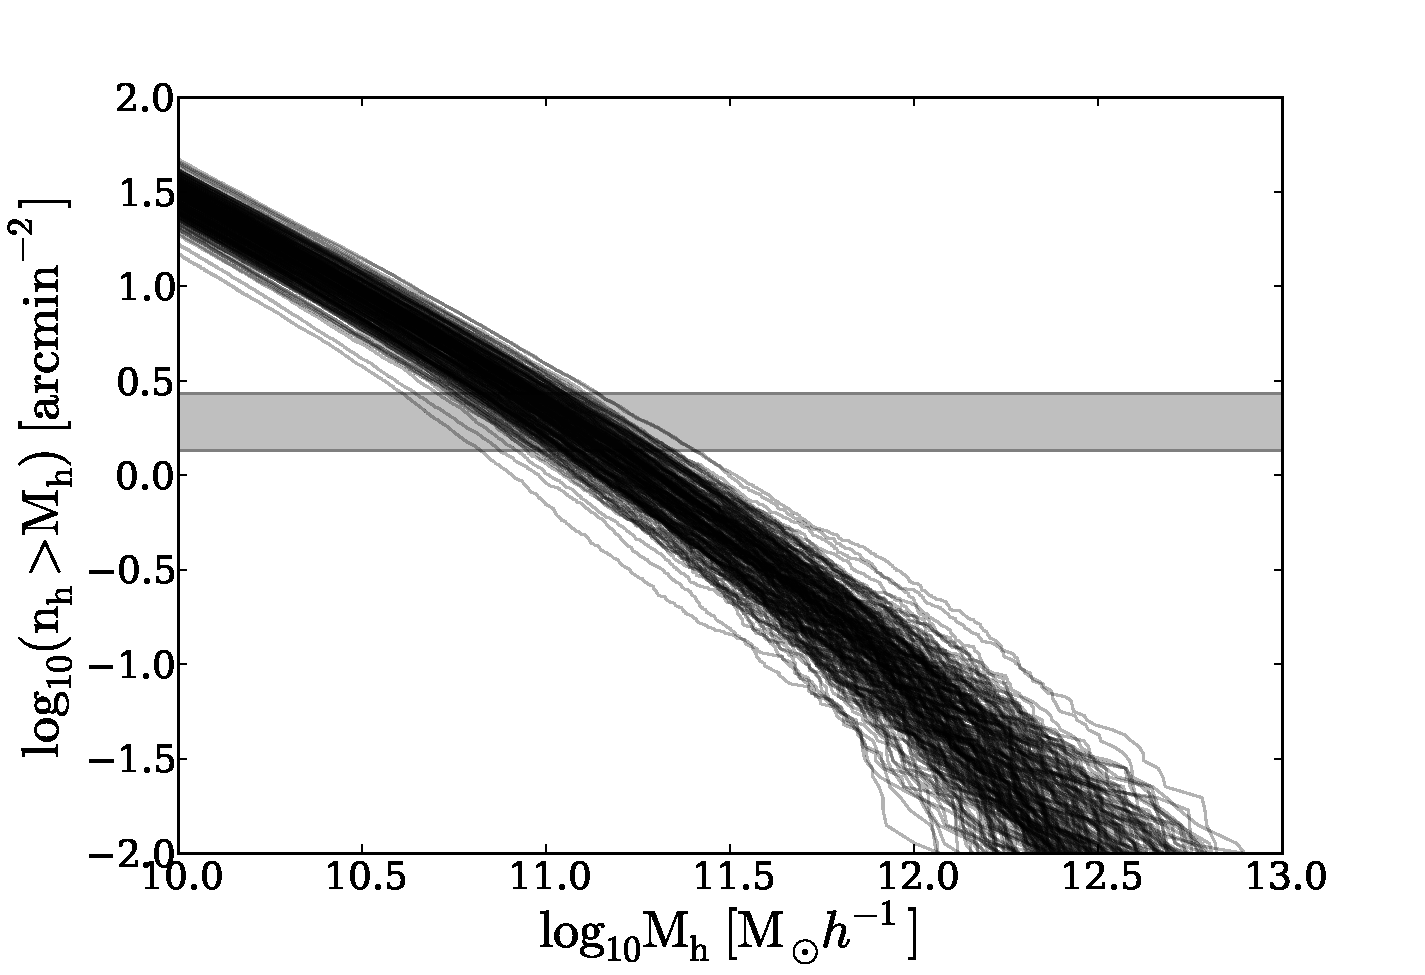
\includegraphics[width=1.00\linewidth,angle=0]{./plots/Fig1.pdf}
\caption{ \label{figure:laes_dist} Cumulative mass function of dark
  matter haloes in the $210$ sub-volumes of $46\times 35\times 41$
  $h^{-3}Mpc^{3}$. The variation in the total number of dark matter
  halos per sub-volume  evidences the effect of cosmic variance at
  such sub-volume scale. It is also appreciable the low population
  $\lesssim10^{-3}h^{2}Mpc^{-2}$ of halos with
  $log(M/M_{\odot})>12.0$}. 
\end{center} 
\end{figure}


\subsection{Dark Matter Halo Number Density}
In Figure \ref{fig:laes_dist} we present the results for  the intergrated dark matter halo surface
density as a function of halos mass for each one of the 210 sub-volumes in
the Bolshoi simulation. The continous lines correspond to the
subvolumes. The shadowed area indicates the surface density values for
LAEs allowed by the observations.  

This result allows us to better understand the
expected trends for the LAEs' preferred mass and the occupation
fraction.  From this Figure we can read which models do not have a
chance reproduce the
observations. Regions in the plot where the halo surface density
values are below the observational constraint correspond to high
masses halo masses. For a LAE model ${\mathcal M}$ with a minimum mass
$M_{\rm   min}> 3 \times 10^{11}$\hMsun located in that mass range,
the surface density is too low compared with observations. 

Conversely, there are regions in the plot where the halo surface
density is always higher than the observational constraints correspond
to models ${\mathcal M}$ with a minimum mass below $M_{\rm min}<
3\times 10^{10}$\hMsun. Models with this minimum mass hava a chance
for successfuly reproducing observations if the occupation fraction
$f_{\rm occ}<1$ is tuned as to lower the halo number density down to
the observed value.    

\subsection{Selection of the preferred halo mass}

\begin{figure*}
\begin{center}
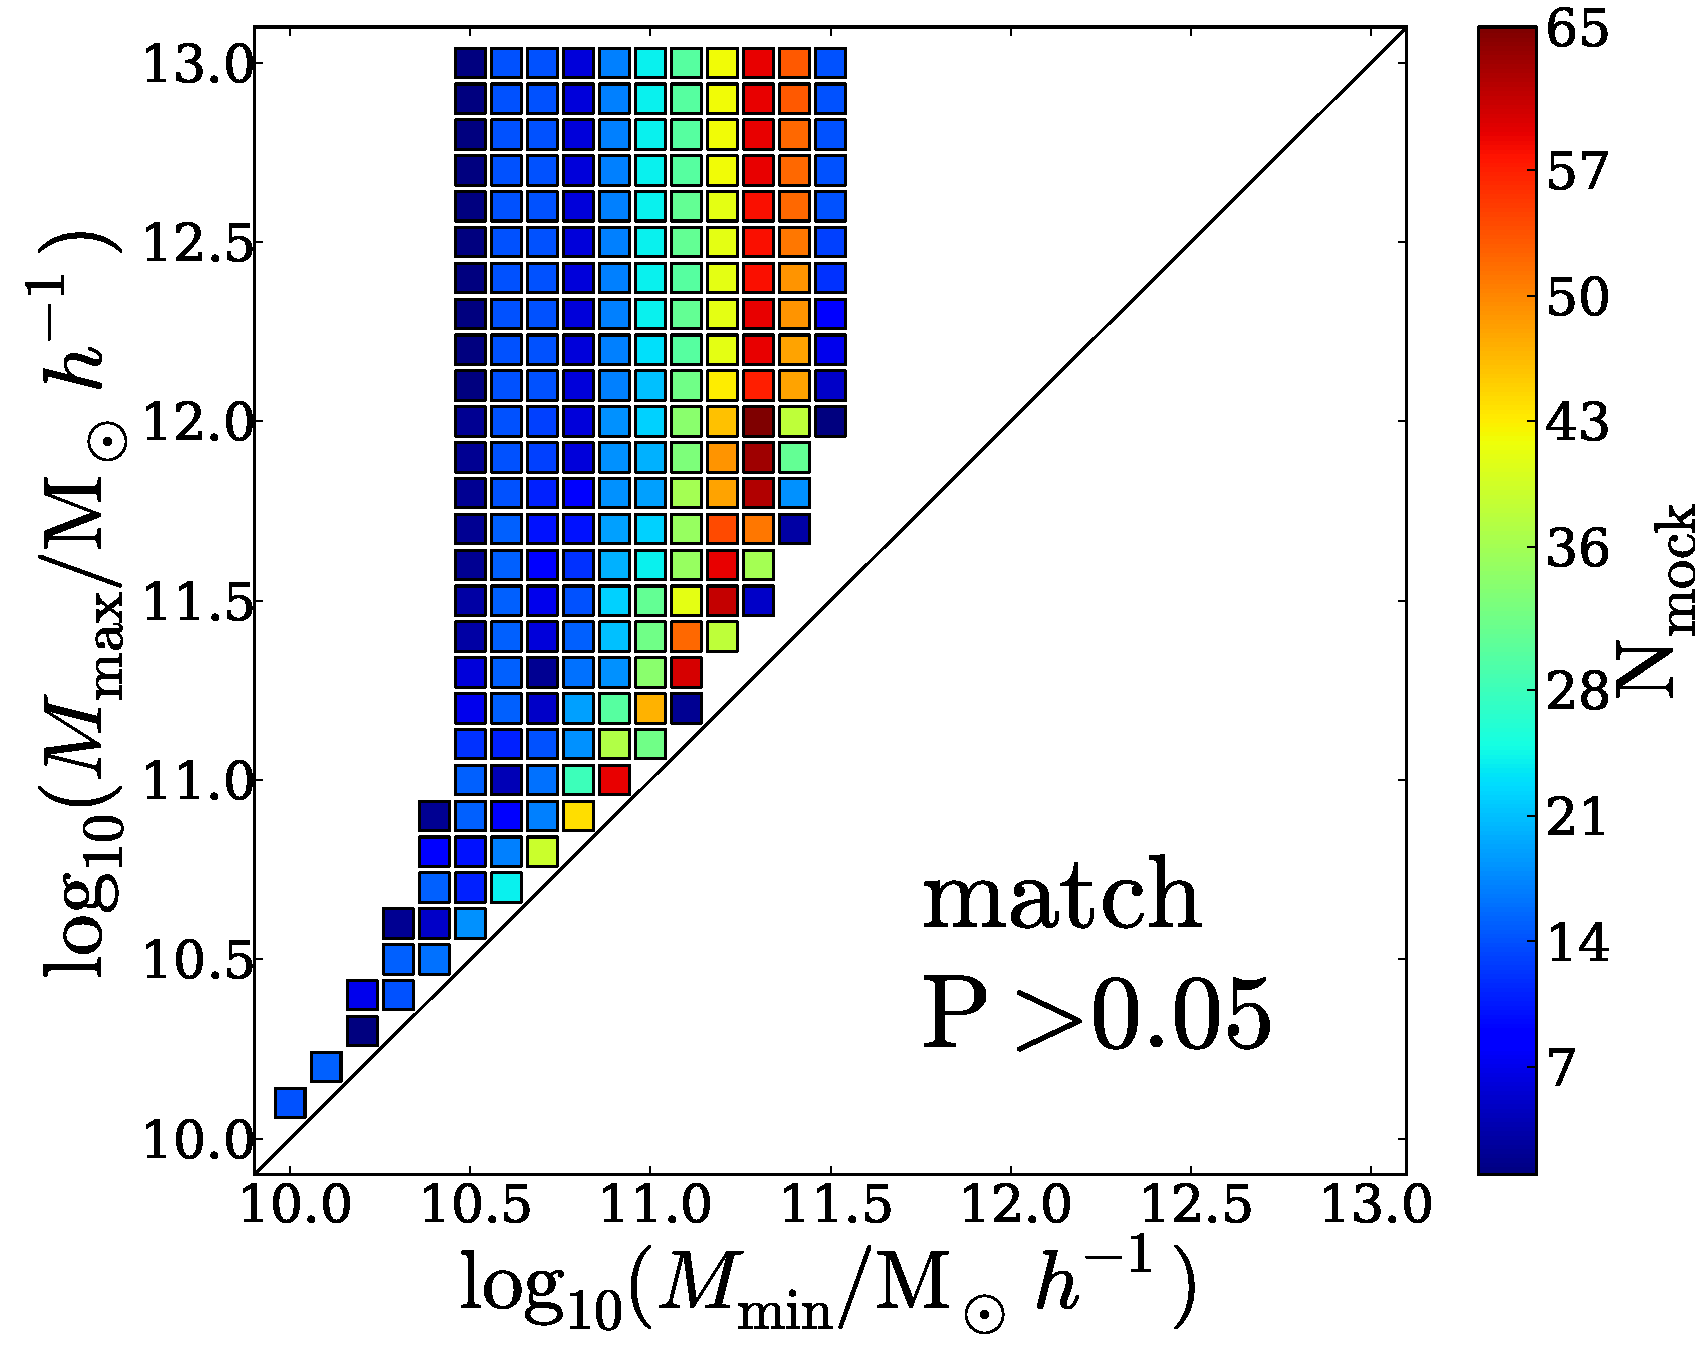
\includegraphics[width=0.46\linewidth,angle=0]{./plots/Fig2_match_P5.pdf}
\hspace{5mm}
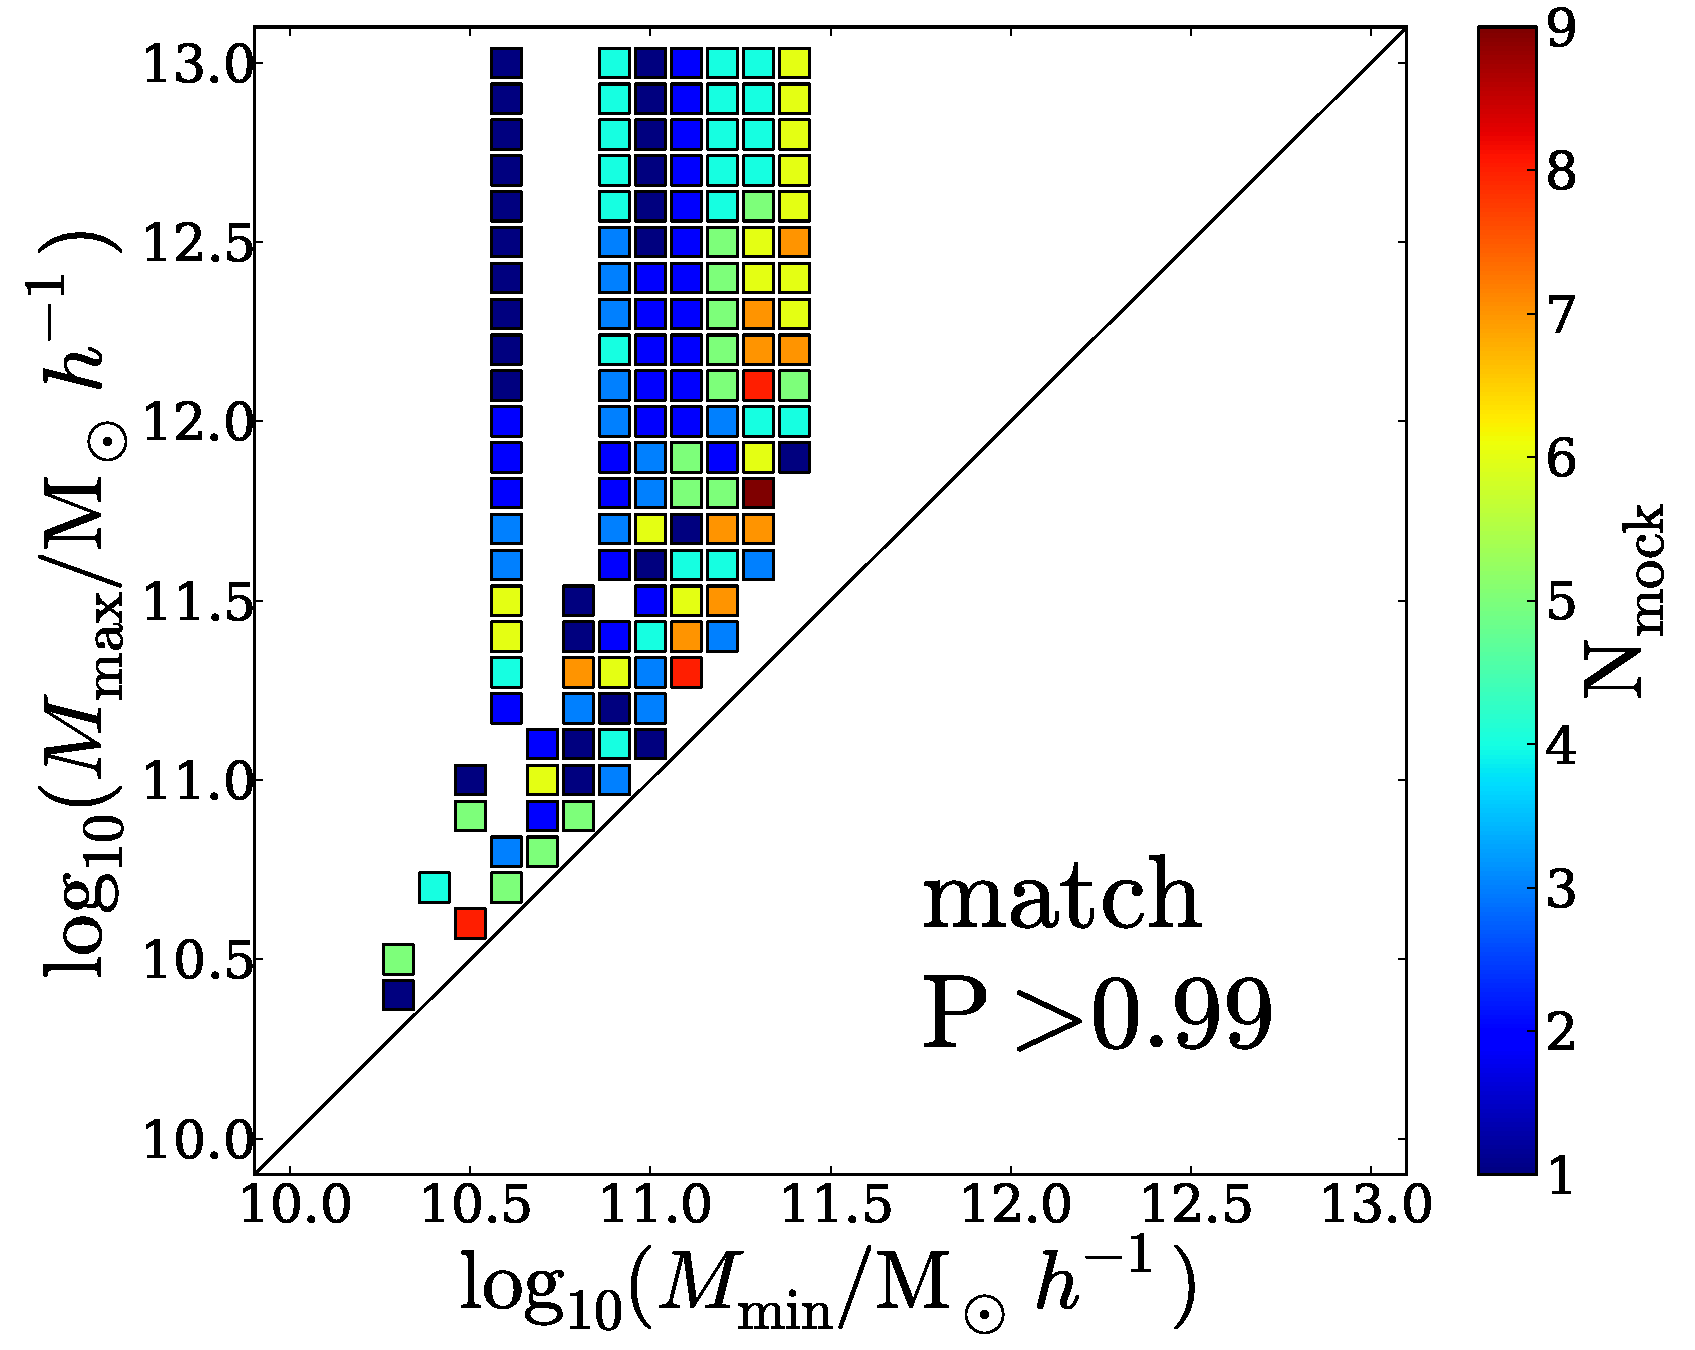
\includegraphics[width=0.46\linewidth,angle=0]{./plots/Fig2_match_P99.pdf}\\
\vspace{5mm}
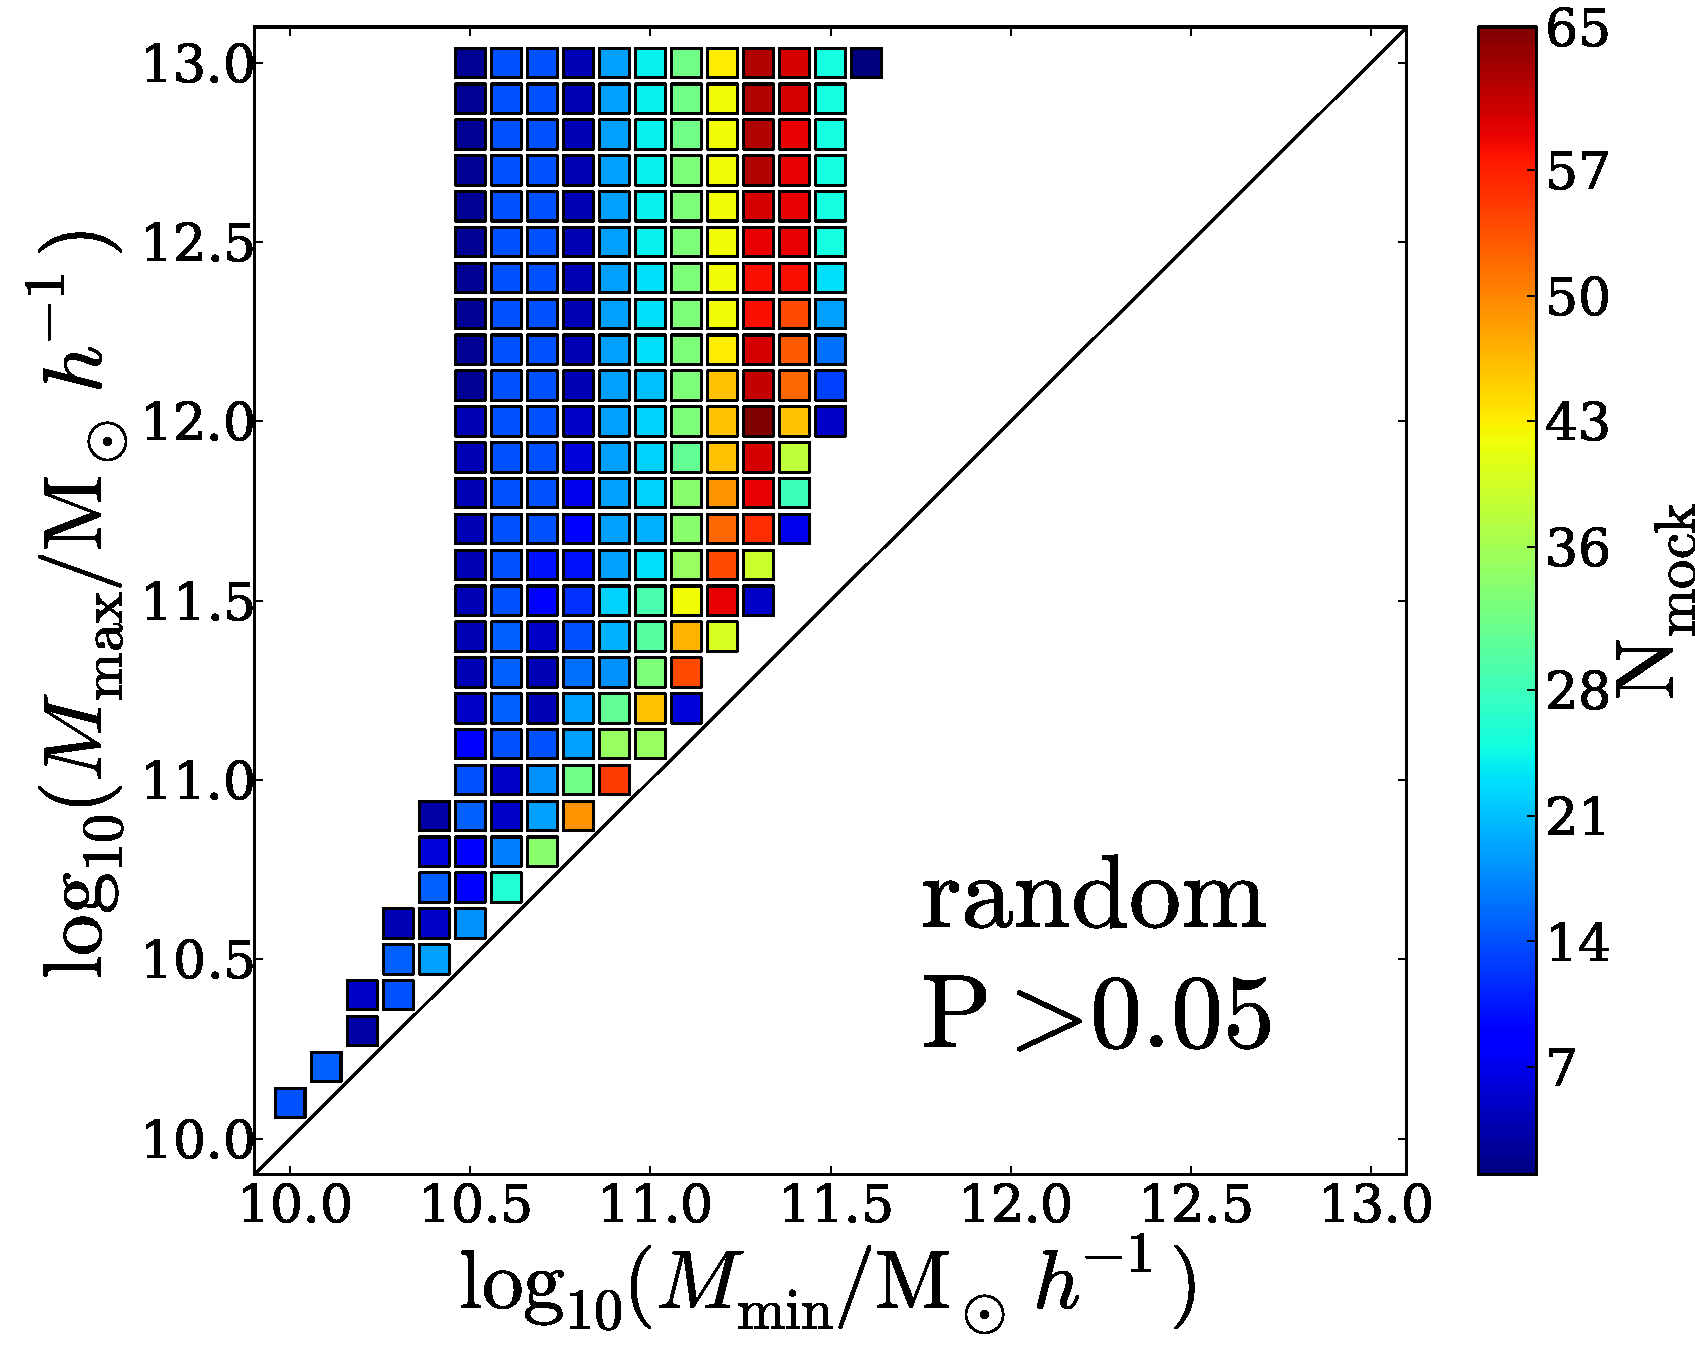
\includegraphics[width=0.46\linewidth,angle=0]{./plots/Fig2_random_P5.pdf}
\hspace{5mm}
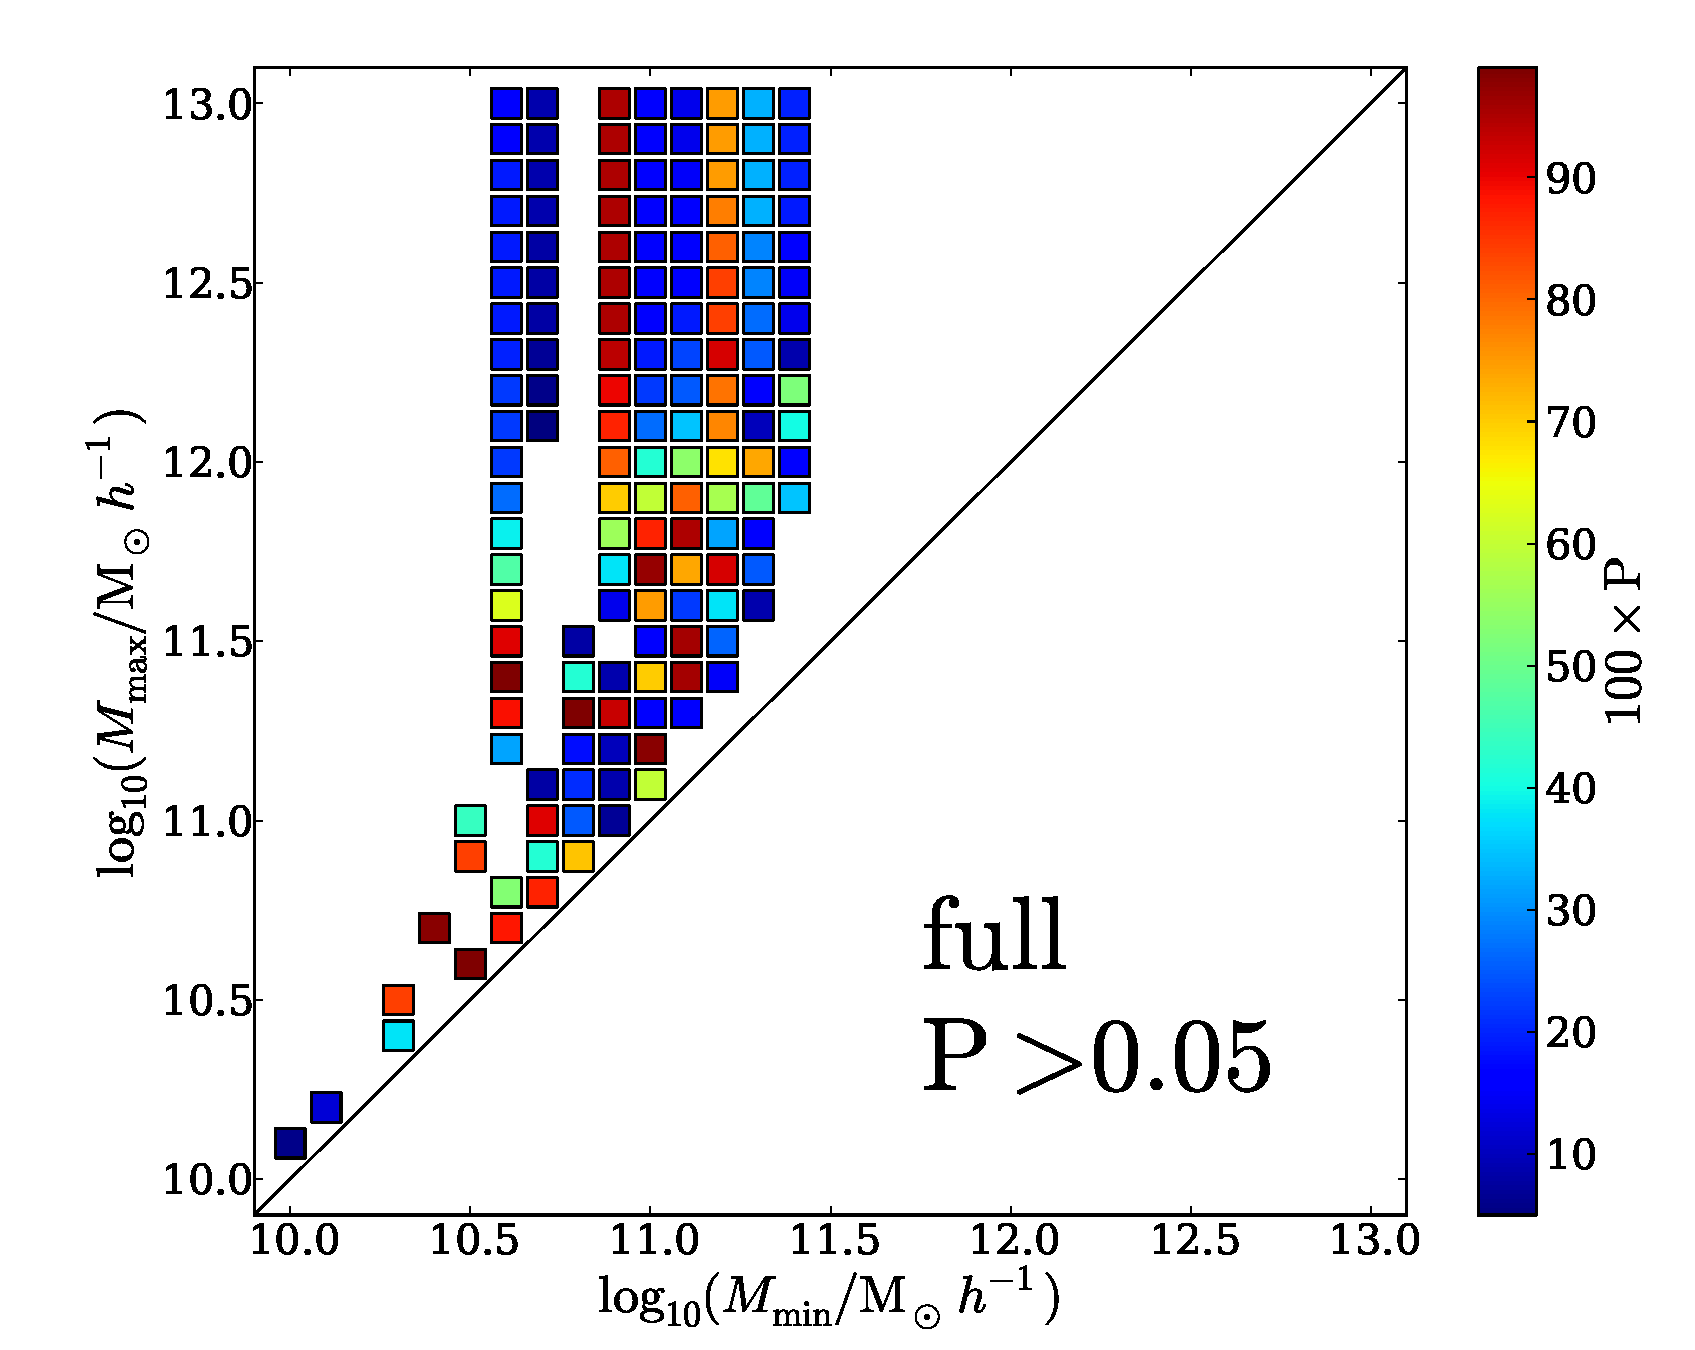
\includegraphics[width=0.46\linewidth,angle=0]{./plots/Fig2_full_P5.pdf}
\end{center} 
\caption{$M_{\rm min}$-$M_{\rm max}$ plane for all models with
  $P>0.05$\label{figure:landscape}.} 
\end{figure*}

Figure \label{figure:landscape} presents the regions in the parameter
space $M_{\rm min}-M_{\rm max}$ where the KS test yields values of
$P>0.1$. Each panel corresponds to the three different ways of
grouping the mock fields. In the case of the methods {\tt{Match}}
and {\tt{Random}} the color code indicates the fraction of these 15
mock surveys with with $P>0.1$. The third panel shows the result for
the method {\tt{Full}}, in this case the color code correspond
to the value of $P$ for a given model.  

These results distinguish three mass regimes. In the first regime, at
high mass values, we find that LAE models with minimum mass of $M_{\rm
  min}>3\times 10^{11}$\hMsun are not compatible with observations as
expected from the analysis in the previous subsection. For masses below $M_{\rm
  min}=3\times 10^{10}$ any values for $M_{\rm min}$ and $M_{\rm max}$
can be made compatible with observations, provided that
$f_{\rm occ}$ is fine tuned to do it. In an intermediate mass regime,
for minimum mass values $3\times 10^{10}\hMsun < M_{\rm min}< 3\times 10^{11}\hMsun$ only a
limited range of models with $M_{\rm max}$ with occupation fraction
$f_{\rm occ}\sim 1$ is able to reproduce observations. 

In these three different mass regimes the occupation monotonically
decreases as a function of the minimum halo mass $M_{\rm min}$. In
Figure XXX we show this treend in three panels following the same
correspondence as Figure XXX. From these results we interpret that the
different mass regimes that were identified correspond to best fit
models with $f_{\rm occ}\sim 1$, $0<f_{\rm occ}<1$ and $f_{\rm
  occ}\sim 0$, respectively. 


The two {\tt match} and {\tt random} methods present the highest
number of matching mock surveys in the medium mass regime. However, it
is important to keep in mind that not all the mock surveys for a
sucessful model ${\mathrm M}$ present a high value $P>0.1$, only a
modest seems to be consistent with observations. This shows that the
cosmic variance is still present on the physical scales probed by
observations. 

To illustrate this point, in Figure \ref{fig:mocks} we present the
results for two mock fields for the {\tt{Match}} method for a model
with the same parameters, but two extreme values for the KS test. 


Conversely there are different models where the KS test yield values of
$P\sim 1$. To illustrate the kind of success represented by these
models, we have selected these best ones in the case of the method
{\tt{MatchObs}}. Figure XXX shows in the main panel the spatial
distribution of the mock surveys, the smaller panel shows the
corresponding surface density distribution and the observational
constraint.  



\subsection{Estimating the Galaxy Bias from the Halo Masses}
Using the results from the previous sections it is possible to infre
the bias of $z\sim 3$ LAEs. Considering a number of $N_{\rm fields}$
the expected number density of galaxies around the region located at
$x_{i}$ is $n_{i}=\bar{n}[1+ b\delta_{\rm DM}(x_{i})]$, where
$\bar{n}$ is the average galaxy number density and $\delta_{\rm
  DM}\equiv (\rho - \bar{\rho})/\bar{\rho}$ is the matter overdensity
in the field [REF robertson]. 

We calculate the bias for each mock catalog in the best models using
the corresponding dark matter overdensity in the simulation. This
results in a distribution of bias values for each model. The results
for this calculation are presented in Figure XX.  We compare this
resul agains the following estimation $b^{2}\sim {\sigma_{N}^{2} -
  \bar{N}}/\bar{N}^{2}\sigma_{\rm DM}^{2}$, where $\bar{N}$ is the
average number counts in the $N_{fields}$, $\sigma_{N}$ is their
dispersion and $\sigma_{DM}$ is the matter variance over many survey
volumes. 

\subsection{Prediction for the angular correlation function}

We calculate the angular correlation function (ACF) for the best
models for a mock survey with a total surface area equal to the full
survey by Yamada et al 2012. We compare these results with the
observed ACF reported by Gawiser et al. XXX.  

\begin{figure}
\begin{center}
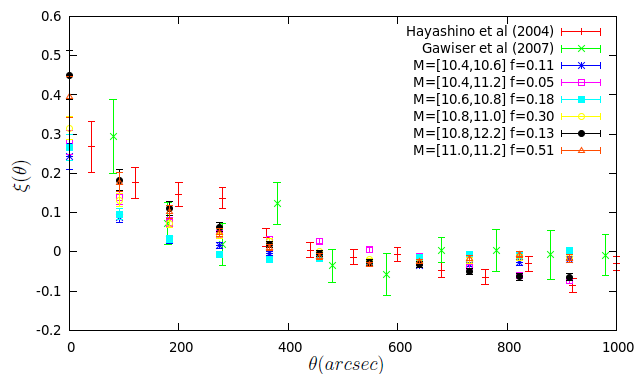
\includegraphics[width=1.00\linewidth,angle=0]{./plots/correlation_best_models_with_obs_comp.png} 
\end{center} 
\caption{ \label{figure:landscape} 
}
\end{figure}


\section{Conclusions}
In this Letter we have constrained the preferred mass for dark matter
halos hosting Lyman Alpha Emitters at a redshift $z=3.1$. We use a
method that matches the cosmic variance in the surface
density number of LAEs from differente observed fields. From this we
are able to constrain the mass range of dark matter halos hosting LAEs
to be in the range $<M_{\rm h}<$ and a corresponding occupation fraction
that escales as $f_{\rm occ} = M_{\rm min}$ with the minium halo mass
defining the halo mass range.

In this letter, this estimate is based on a large Nbody simulation
where we select a range a fraction of halos in a given mass range to
host LAEs. We explicitly construct mock observations to derive
statistics that can be compared against observations. 

 The method is based on making an estimate of the cosmic
variance from different observed fields. Based on a Nbody simulation,
we select the range of halo masses, $M_{\rm min}<M_{\rm h}<M_{\rm
  max}$, and the fraction of these halos, $f_{\rm occ}$, that could
host LAEs being compatible witht the cosmic variance constraints.

We have used a large volume cosmological N-body simulation that allows
us to extract $210$ sub-boxes each of which has a comparable
volume to the field of view observed by Yamada et al. 2012. The
comparison of the observed number density distribution against the
results from our model is based on three different ways of
constructing mock surveys. The first reproduces the spatial
correlation between the $12$ observational fields, the second breaks
this spatial correlation while keeping the number of fields and the
third one simply includes all the $210$ sub-boxes.



\section*{Acknowledgments} 


\bibliographystyle{mn2e}
\bibliography{references} 

\end{document}

